\begin{thm}{067}{\hosi 4}{進研模試 数学A}
 $\triangle\mr{ABC}$について、AB$=5$, BC$=3\sqrt{5}$, $\tan\mr{A}=-\dfrac{3}{4}$である。$\angle\mr{BCD}=90^\circ$ かつ CD$=\dfrac{\sqrt{5}}{2}$ である点Dを点Aと同じ側にとり、直線ACと直線BDの交点をEとする。DEの長さを求めよ。
\end{thm}

$\tan\mr{A}<0$より$\angle\mr{A}$は鈍角なので、$\cos\mr{A}<0$である。$1+\tan^2\mr{A}=\dfrac{1}{\cos^2\mr{A}}$から、$\cos\mr{A}=-\dfrac{4}{5}$である。続いて余弦定理により
\[ \mr{BC}^2=\mr{AB}^2+\mr{AC}^2-2\mr{AB}\cdot\mr{AC}\cos\mr{A} \,dou\, \mr{AC}^2+8\mr{AC}-20=0 \]
よってAC$=2$がわかる。さらに余弦定理から
\[ \cos\mr{C}=\frac{\mr{AC}^2+\mr{BC}^2-\mr{AB}^2}{2\mr{AC}\cdot\mr{BC}} = \frac{2}{\sqrt{5}} \]
が得られる。さらに$\cos$と$\tan$の相互関係から、$\tan\mr{C}=\dfrac{1}{2}$となる ($\angle\mr{C}$は明らかに鋭角)。

点Bを通りBCに垂直な直線と、ACの交点をFとする。
\begin{figure}[H]
 \centering
 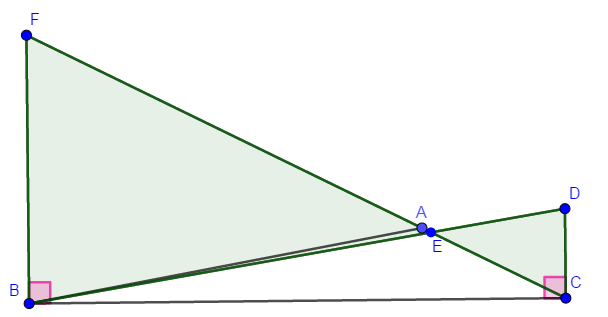
\includegraphics[width=0.8\linewidth]{../problems/Q_067/A_067.png}
\end{figure}
直角三角形CBFを考えると、
\[ \tan\mr{C}=\frac{\mr{FB}}{\mr{BC}}=\frac{1}{2} \]
となっているから、FB$=\dfrac{3\sqrt{5}}{2}$。一方FBとDCは平行で、$\triangle\mr{BFE}\sim\triangle\mr{DCE}$であって、相似比は$\mr{FB}:\mr{CD}=\dfrac{3\sqrt{5}}{2}:\dfrac{\sqrt{5}}{2}=3:1$。よって$\mr{BE}:\mr{DE}=3:1$とわかって、
\[ \mr{DE}=\frac{1}{4}\mr{BD}=\frac{1}{4}\sqrt{\mr{BC}^2+\mr{CD}^2}=\frac{\sqrt{185}}{8} \]